% =============================================================================
% COPYRIGHT AND DISCLAIMER
% =============================================================================
% This file is provided as a convenience template for competition participants.
% By using it, you accept full responsibility for compliance with all applicable
% copyright, licensing, and usage rules of the Association for Computing
% Machinery (ACM) and of any LaTeX packages you load (including, without
% limitation, the "acmart" document class and related ACM materials).
%
% Consult ACM's official publication, template, and copyright policies before
% using this setup for any purpose other than this competition. Do not assume
% that this template may be reused, redistributed, or submitted elsewhere
% without independently verifying ACM's current rules.
%
% Use of the "acmart" class, the "sigconf" option, or ACM-style formatting in
% this template does NOT mean that this report, this competition, its organizers,
% or any resulting PDF is sponsored, endorsed, affiliated with, or published by
% ACM. ACM trademarks and branding remain the property of ACM.
%
% Template packages live in preamble.tex.
% Citations live in main.bib (template) and refs_extra.bib (this repository).
% =============================================================================

\documentclass[sigconf]{acmart}
\input{preamble}

% Guide styling: \guideStyletrue = show gray italic hints; \guideStylefalse = omit them
% \guideStyletrue
\guideStylefalse

\begin{document}

\title{ResNet-34 U-Net with a Skeleton-Aware Loss for Full-Disk Solar Filament Segmentation}
\subtitle{A Solution to the Solar Filament Segmentation Challenge 2026} % DO NOT CHANGE

\author{Nguyen Van Son}
\affiliation{%
  \institution{FPT University}
  \city{Hanoi}
  \country{Vietnam}
}
\email{dzson231@gmail.com}

\begin{abstract}
    This report describes our solution to the Solar Filament Segmentation Challenge~2026, a Kaggle competition on automatic segmentation of solar filaments in GONG H-$\alpha$ observations. We train a ResNet-34 U-Net with a Dice, cross-entropy and soft-skeleton clDice loss on $512\times512$ crops centred on annotated filaments, apply it to full-disk images with four-view flip test-time augmentation, and obtain filament instances as connected components of the thresholded probability map. On 141 held-out validation images the released pipeline reaches a Panoptic Quality of 0.108 (95\% bootstrap interval 0.091--0.126) and a mean pixel Dice of 0.346 (0.313--0.378). It is a faithful, reproducible baseline, not a competitive full-disk solution, and it is not the process that produced our leaderboard entry; we state this relation explicitly in Section~\ref{sec:evaluation}.
\end{abstract}

\maketitle

% ==================================== %
%              INTRODUCTION            %
% ==================================== %
\section{Introduction}
    This report goes over the details of our submitted solution to the Solar Filament Segmentation Challenge~2026 \cite{filament-segmentation-2026}. The challenge, launched on July~10,~2026, is organized by the Earth-Space AI Research (ESAIR) Lab\footnote{\href{https://www.esairlab.com/home}{www.esairlab.com/}}. This challenge utilizes the MAGFiLO dataset for evaluation of the segmentation algorithms \cite{ahmadzadeh2024dataset}. We participated as Team Kaiser (Kaggle handle \texttt{snnguynvnk19hl}). Instances are scored with Panoptic Quality (PQ) \cite{kirillov2019panoptic}, so a method must detect each filament as one object (IoU\,$>$\,0.5); fragmenting or merging filaments is penalised even when pixel overlap is high. All code, the trained weights, pinned requirements and a notebook that reproduces the predictions without re-training are in the repository\footnote{\url{https://github.com/snnguynvnk19hl/solar-filament-segmentation-2026}}.


% ==================================== %
%              METHODOLOGY             %
% ==================================== %
\section{Methodology}\label{sec:methodology}

\subsection{Data and sampling strategy}
The released pipeline uses only the competition training split (707 annotated $2048\times2048$ images) and no external data or additional ground-truth metadata. Images are sorted by file name; the first 566 images (7,522 annotated filaments) are used for training and the last 20\% (141 images, 677 filaments) form the validation set. The split is by image, so all filaments of one image fall on the same side. The 180 test images are used only to generate predictions; no test image or test label was used to fit or select anything in this pipeline. The post-processing parameters (threshold, minimum area, input size) were selected on the validation images.

\subsection{End-to-end pipeline}
Figure~\ref{fig:pipeline} summarises the pipeline.

\begin{figure*}[t]
    \centering
    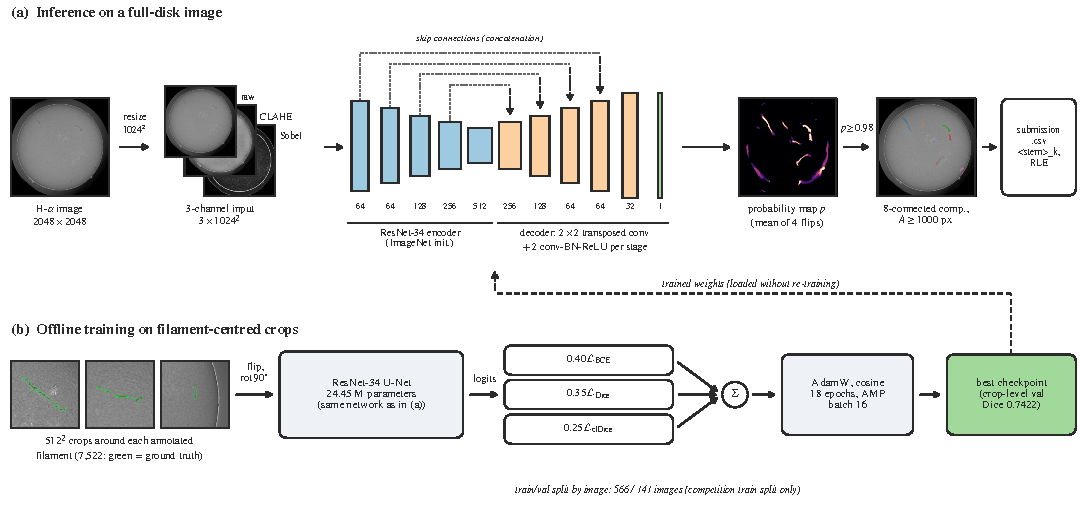
\includegraphics[width=0.97\textwidth]{figures/pipeline.pdf}
    \caption{Pipeline. (a)~Inference on a full-disk image; the thumbnails are produced by the released code and weights (block height indicates spatial resolution, numbers give channel counts; the Sobel channel is contrast-enhanced for display). (b)~Offline training on filament-centred crops (green: ground truth); the resulting weights are loaded, not re-trained, at inference time (dashed arrow).}
    \label{fig:pipeline}
\end{figure*}

\paragraph{Pre-processing.} The image is converted to grayscale and resized to $1024\times1024$ (area interpolation). Three channels in $[0,1]$ are stacked: the raw intensity, a CLAHE-equalised version (clip limit 2.0, $8\times8$ tiles) \cite{zuiderveld1994clahe}, and the Sobel gradient magnitude normalised by its maximum. CLAHE reduces limb darkening and station-dependent contrast; the gradient channel emphasises filament boundaries.

\paragraph{Network.} An ImageNet-initialised ResNet-34 encoder \cite{he2016resnet} is combined with a U-Net-style decoder \cite{ronneberger2015unet}: four transposed-convolution up-sampling stages with skip connections (two $3\times3$ conv--BN--ReLU layers each), a final up-sampling to input resolution and a $1\times1$ convolution that outputs one logit per pixel (24.45\,M parameters).

\paragraph{Training.} A training sample is a $512\times512$ crop centred on one annotated filament (side $\max(1.4\cdot\text{box size},512)$ pixels resized to 512, centre jittered by up to one sixth of the box), with random flips and $90^\circ$ rotations. The loss is $0.40\,\mathcal{L}_{\mathrm{BCE}}+0.35\,\mathcal{L}_{\mathrm{Dice}}+0.25\,\mathcal{L}_{\mathrm{clDice}}$, where the soft-skeleton clDice term \cite{shit2021cldice} (three skeletonisation iterations) penalises breaks of the thin filament spine more than an overlap loss. We use AdamW \cite{loshchilov2019adamw} (learning rate $3\cdot10^{-4}$, weight decay $10^{-4}$), a cosine schedule to $10^{-6}$, batch size 16, 18 epochs, mixed precision and seed 2026. The checkpoint with the highest \emph{crop-level} validation Dice (0.7422, epoch 18) is released.

\paragraph{Inference and post-processing.} The full disk is resized to $1024\times1024$ and passed through the network in four views (identity, horizontal, vertical and both flips); the sigmoid outputs are averaged and bilinearly resized to $2048\times2048$. Pixels with probability $\ge\tau$ form a binary mask whose 8-connected components are the predicted filaments; components smaller than $A$ pixels are discarded. Connected components are pixel-disjoint, so instances never overlap. Each instance is written as compressed COCO RLE. We select $\tau=0.98$ and $A=1000$ on the validation images. Inference takes about 0.6\,s per image on a laptop RTX 4060 GPU.


% ==================================== %
%              EVALUATION              %
% ==================================== %
\section{Evaluation}\label{sec:evaluation}

\subsection{Evaluation strategy}
We evaluate on the 141 held-out validation images with (i) Panoptic Quality with its components SQ and RQ (IoU\,$>$\,0.5, one-to-one matching, pooled over images) and (ii) the mean per-image pixel Dice between the union of ground-truth and predicted filaments. We also count fragmentation: \emph{1:N} is the number of ground-truth filaments that contain at least half of the area of two or more predictions, and \emph{N:1} the number of predictions that cover at least half of two or more ground-truth filaments. Uncertainty is given as 95\% percentile bootstrap intervals over images (2,000 resamples). Our PQ and fragmentation counts are our own implementation and may differ in details from the official scorer. Because $\tau$ and $A$ were chosen on these images, the best row is optimistic.

\begin{table*}[t]
    \caption{Full-disk validation (141 images, 677 filaments), $1024\times1024$ input, four-view TTA, no opening. PQ and Dice are point estimates with 95\% bootstrap intervals over images; $\tau$ is the probability threshold and $A$ the minimum instance area in pixels. The last row is the selected configuration.}
    \label{tab:val}
    \centering
    \small
    \begin{tabular}{ccccccccc}
        \toprule
        $\tau$ & $A$ & PQ [95\% CI] & SQ & RQ & Dice [95\% CI] & TP/FP/FN & 1:N & N:1 \\
        \midrule
        0.5 & 60 & 0.020 [0.013, 0.028] & 0.593 & 0.034 & 0.199 [0.176, 0.224] & 29/1014/648 & 0 & 156 \\
        0.5 & 1000 & 0.022 [0.014, 0.030] & 0.593 & 0.037 & 0.200 [0.177, 0.226] & 29/854/648 & 0 & 156 \\
        0.8 & 60 & 0.056 [0.044, 0.069] & 0.597 & 0.094 & 0.300 [0.271, 0.329] & 72/783/605 & 0 & 148 \\
        0.8 & 1000 & 0.059 [0.046, 0.073] & 0.597 & 0.099 & 0.302 [0.274, 0.332] & 71/682/606 & 0 & 147 \\
        0.9 & 60 & 0.074 [0.060, 0.087] & 0.600 & 0.123 & 0.317 [0.287, 0.347] & 94/761/583 & 0 & 145 \\
        0.9 & 1000 & 0.077 [0.063, 0.092] & 0.601 & 0.129 & 0.319 [0.290, 0.349] & 91/647/586 & 0 & 144 \\
        0.95 & 60 & 0.084 [0.069, 0.098] & 0.612 & 0.137 & 0.330 [0.299, 0.360] & 105/754/572 & 1 & 140 \\
        0.95 & 1000 & 0.089 [0.073, 0.105] & 0.611 & 0.146 & 0.332 [0.302, 0.363] & 102/622/575 & 1 & 138 \\
        0.98 & 60 & 0.101 [0.086, 0.117] & 0.617 & 0.164 & 0.349 [0.318, 0.380] & 126/734/551 & 1 & 139 \\
        \textbf{0.98} & \textbf{1000} & \textbf{0.108 [0.091, 0.126]} & \textbf{0.618} & \textbf{0.175} & \textbf{0.346 [0.313, 0.378]} & \textbf{119/565/558} & \textbf{1} & \textbf{136} \\
        \bottomrule
    \end{tabular}
\end{table*}

\subsection{Results}
Table~\ref{tab:val} shows that the full-disk quality of the released pipeline is low. Raising the threshold removes many false positives and is the largest single improvement (PQ from 0.020 at $\tau=0.5$ to 0.108 at $\tau=0.98$); a larger minimum area helps slightly. The best value lies at the edge of the explored threshold grid, and higher thresholds were not explored. Running the network at a higher input resolution makes things worse: at the same settings ($\tau=0.9$, $A=1000$) PQ falls from 0.077 at $1024^2$ to 0.053 at $1536^2$ and 0.032 at $2048^2$ because the number of false-positive components grows from 647 to 1,812 and 3,738, so we kept $1024^2$. The mean matched IoU (SQ) is about 0.6 in all settings, i.e.\ the detected filaments are segmented reasonably well; the loss is in recognition (RQ). Fragmentation (1:N) is at most one case in every setting, whereas merging (N:1) involves 136 to 156 predictions. Evaluated on training-style crops centred on filaments, the same checkpoint reaches a Dice of about 0.76 (0.7422 on all 677 validation crops), which confirms that the implementation matches the training setup and that the weakness comes from applying a crop-trained model to whole images.

Figure~\ref{fig:examples} shows validation examples at the 90th, 50th and 10th percentile of the per-image Dice.

\begin{figure*}[t]
    \centering
    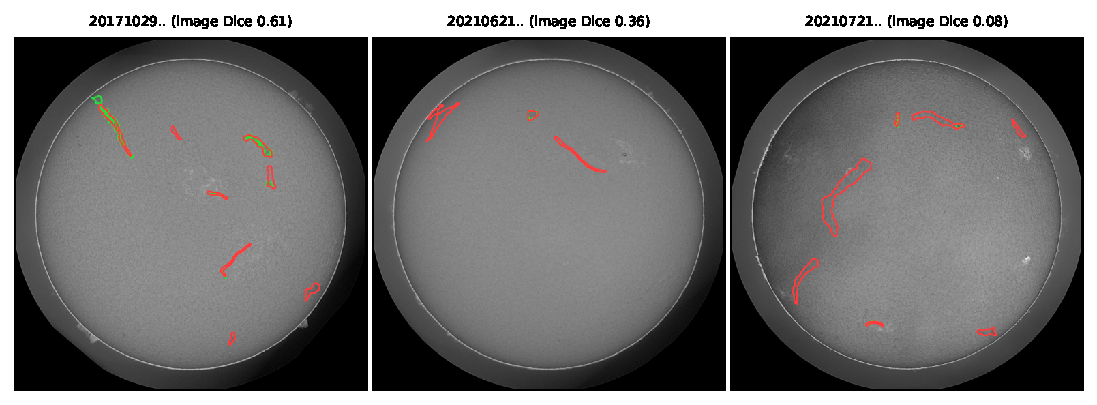
\includegraphics[width=0.97\textwidth]{figures/examples.pdf}
    \caption{Validation examples at the 90th, 50th and 10th percentile of per-image Dice, with ground-truth (green) and predicted (red) filament contours drawn on the same image.}
    \label{fig:examples}
\end{figure*}

\subsection{Relation to our leaderboard entry}
Our final leaderboard submission (reference 58173877; public and private score 0.55; rank 38 of 1,567 on the public leaderboard of 2026-11-17) was obtained by a multi-stage chain of experiments in which earlier prediction files were combined and post-processed instance by instance. That chain is not part of the repository and cannot be regenerated by its code. The predictions of the released pipeline (\texttt{predict.py}) were not submitted to the leaderboard, and we therefore make no claim that the repository reproduces the leaderboard score; the validation results above are the evidence for the released pipeline.

\subsection{Strengths, weaknesses and possible improvements}
\textbf{Strengths:} a small, fully specified model (24.45\,M parameters, 0.6\,s per image) that is trained only on the competition training data, with a documented split, pinned dependencies, weights in the repository and a validated, overlap-free output format. The matched filaments have an SQ of about 0.6. \textbf{Weaknesses:} the model is trained on single-filament crops that always contain a filament, but is applied to whole discs, which produces many false-positive components and merges neighbouring structures (N:1 is large); instances are separated only by connected components; a single split and seed were used. \textbf{Improvements:} train on full-disk tiles that include negative regions or hard-negative mining, add an instance-aware head or a learned merge/split step guided by the filament spine, calibrate the probabilities per observing station, and use cross-validation with several seeds to obtain tighter estimates.


% ==================================== %
%            ACKNOWLEDGMENT            %
% ==================================== %
\section{Acknowledgment}\label{sec:acknowledgment}
    % Do not change
    The organization of the Filament Segmentation Challenge 2026 is partially supported by the U.S. National Science Foundation (NSF) under Grant No. 2209912 and 2433781, directorate for Computer and Information Science and Engineering (CSE), and Office of Advanced Cyberinfrastructure (OAC), and Grant No. 2511630, AST Division Of Astronomical Sciences and MPS Directorate for Mathematical and Physical Sciences.

    The Filament Segmentation Challenge 2026 is sponsored by the U.S. National Science Foundation (NSF) National Solar Observatory (NSO).

    This work utilizes GONG data obtained by the NSO Integrated Synoptic Program, managed by the National Solar Observatory, which is operated by the Association of Universities for Research in Astronomy (AURA), Inc. under a cooperative agreement with the National Science Foundation and with contribution from the National Oceanic and Atmospheric Administration. The GONG network of instruments is hosted by the Big Bear Solar Observatory, High Altitude Observatory, Learmonth Solar Observatory, Udaipur Solar Observatory, Instituto de Astrofísica de Canarias, and Cerro Tololo Interamerican Observatory.

\bibliographystyle{ACM-Reference-Format}
\bibliography{main,refs_extra}

\end{document}
